\documentclass{article}
\usepackage[T1]{fontenc}
\usepackage{microtype,graphicx,booktabs,amsmath}
\usepackage[hypertexnames=false]{hyperref}
\usepackage[accepted]{mlsys2025}
\hypersetup{pdftitle={A Study of Prefix Sharing in LLM Serving},pdfsubject={Rice University COMP536 final project},pdfauthor={Thomas Lin; Yu-Ting Chung; Patrick Chiou; Yu-Xin Lai}}
\mlsystitlerunning{A Study of Prefix Sharing in LLM Serving}
\makeatletter
\renewcommand{\Notice@String}{Rice University, COMP536 course project, November 2026; updated November 27.}
\renewcommand{\printAffiliationsAndNotice}[1]{\begingroup\renewcommand{\thefootnote}{}\footnotetext{\textsuperscript{1}Rice University. \Notice@String}\endgroup}
\makeatother
\begin{document}
\twocolumn[
\mlsystitle{A Study of Prefix Sharing in LLM Serving}
\begin{mlsysauthorlist}
\mlsysauthor{Thomas Lin}{rice}
\mlsysauthor{Yu-Ting Chung}{rice}
\mlsysauthor{Patrick Chiou}{rice}
\mlsysauthor{Yu-Xin Lai}{rice}
\end{mlsysauthorlist}
\mlsysaffiliation{rice}{Rice University}
\begin{center}\small \texttt{tl183@rice.edu, yc223@rice.edu, pc82@rice.edu, yl371@rice.edu}\end{center}
\vskip .08in
\begin{abstract}
Prefix caching avoids repeated prefill work, but its effectiveness depends on capacity, block granularity and workload locality. We implement a CPU trace executor within vLLM v0's online serving path, retaining scheduling, sequence management and virtual prefix-block allocation. We evaluate matched single- and multi-turn ShareGPT workloads over @M2_RUNS@ configurations, reuse a validated eight-source, 51-configuration baseline study, and evaluate eight policies on two mixed-workload compositions. @ABSTRACT_RESULT@ A repository-reported five-mixture sweep adds hold/admission sensitivity. The current simulator passes 153 correctness tests including both API frontends after repairing workload-label transport through multiprocessing. Results characterize realized cache reuse under controlled trace replay rather than GPU latency or throughput; limited production windows and single-seed mixed comparisons constrain generalization.
\end{abstract}
\vskip .12in]
\printAffiliationsAndNotice{}

\section{Introduction}
LLM serving repeatedly processes instructions, documents and conversation histories that share input prefixes. Prefill constructs attention key/value (KV) state; subsequent decoding extends it. Retaining identical full-prefix KV blocks lets later requests avoid redundant prefill. PagedAttention provides block-based memory management and sharing in vLLM \citep{kwon2023}. Which reusable blocks remain available depends on both workload arrival structure and eviction decisions under limited capacity.

Different workloads create different retention problems. Growing conversations often revisit recently extended histories; a common instruction may recur across many otherwise unrelated requests; document questions can concentrate reuse in short bursts. This motivates three questions: can CPU trace replay preserve the online serving control flow, how do capacity and block size affect realized sharing in homogeneous chat, and which eviction rules work across heterogeneous and mixed workloads?

We contribute an online trace executor, causal client and request/block metrics, then compare homogeneous chat, eight separate sources and eight policies under two mixtures. Policy orderings are configuration-specific.

\section{Background and Related Work}
A KV block depends on its preceding token prefix: identical chunks in different histories are not generally interchangeable. Reference-counted active blocks are not candidates for eviction; policies order unused cached content. LRU favors recent access, LFU allocator access frequency, and FIFO insertion order. Their usefulness depends on whether past recency, popularity or insertion age predicts future demand.

vLLM's PagedAttention addresses block allocation and sharing \citep{kwon2023}. SGLang uses RadixAttention for reuse across structured programs \citep{sglang}; Prompt Cache uses explicitly defined reusable modules \citep{promptcache}. CacheBlend addresses non-prefix retrieval chunks with selective recomputation \citep{cacheblend}, whereas our simulator retains exact full-prefix semantics. Mooncake studies KV-centric disaggregated serving \citep{mooncakepaper}; our use of released anonymous hashes does not reproduce its distributed architecture. We study replacement behavior inside an existing serving control path, not a new attention algorithm or GPU serving speedup.

\section{System Design and Implementation}
\subsection{Trace execution within online serving}
The online path preprocesses HTTP prompts, admits/schedules sequences, manages blocks and processes token outputs. Our \texttt{SimExecutor}/\texttt{SimExecutorAsync} replaces model execution with \texttt{Simulator.step}; the surrounding v0 components remain active. Workload metadata and executor selection are modified, so the scheduler is not claimed entirely unchanged. Figure~\ref{fig:architecture} contrasts the execution backends and illustrates exact prefix sharing.

\begin{figure*}[t]
\centering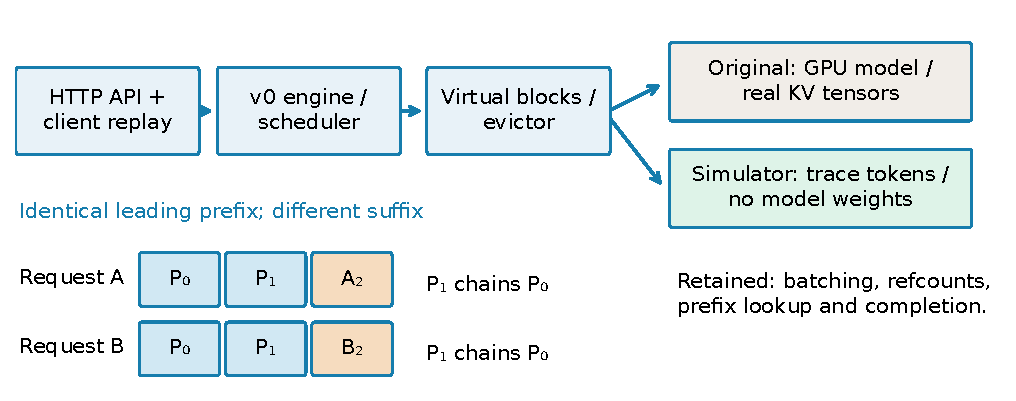
\includegraphics[width=.95\textwidth]{figures/system_prefix.pdf}
\caption{Retained online control path with GPU execution replaced by trace replay. Identical leading token blocks share KV state; a changed suffix is computed separately. Chained identity prevents sharing an identical local block after a different prefix.}
\label{fig:architecture}
\end{figure*}

The simulator consumes scheduled metadata, honors sampling flags and computed blocks, and returns compatible sampler outputs. Next-token selection follows output length, preserving progress after recomputation. Cached prompts recompute the final sampling token. Normal EOS/stop handling releases state; exact prompt tokens plus request IDs distinguish duplicate prompts with different replies.

No model weights, attention kernels or actual KV tensors are loaded. Configuration and tokenizer files remain necessary. Virtual KV bytes per block are
\begin{equation}
B_{\rm KV}=2 L H_{\rm KV}d_h b s,
\end{equation}
where $L$ is attention layers, $H_{\rm KV}$ KV heads per rank, $d_h$ head dimension, $b$ tokens/block and $s$ bytes/element. This geometry controls virtual capacity, not allocated GPU memory. The executor awaits synthetic costs of0.01\,ms per uncached prefill token and0.1\,ms per decode sequence-step. CPU/HTTP overhead and queuing remain real wall time. LoRA, prompt adapters, speculative decoding and multistep scheduling are unsupported in this executor.

\subsection{Client, traces and workload labels}
\texttt{TraceBuilder} reuses serving preprocessing and the model's chat template/tokenizer, with fixed date arguments. ShareGPT normalization enforces role ordering and filters whole conversations for context eligibility. Single-turn mode retains only the first user/reply pair; multi-turn retains all eligible turns. The two modes thus share the same initial conversations and first-turn prompts/target arrivals. Optional agent truncation retains a causal prefix.

The concurrency-limited client uses recorded times or seeded Poisson arrivals and waits for the preceding reply before each later turn. It validates text, token counts and finish reason; failures stop descendants. Dispatch lag distinguishes target from achieved arrivals.

Dataset-provided labels propagate through request, sequence and block metadata; no online workload classifier is implemented. A missing optional label remains \texttt{None}. We repaired an incomplete multiprocessing path by adding the label to the client method, pickled RPC request and engine-side submission, rather than dropping it or disabling the frontend. Both endpoints/frontends pass integrated request/block-label checks. A subsequent fix strips all model-configured stop IDs from recorded replies to avoid premature termination; it changes preparation, not historical prepared traces. Current simulator correctness evidence is153 passing tests, including trace identity, batching, EOS, preemption/recomputation and eviction ordering. This validation is scoped to the simulator suite, not all GPU-dependent upstream tests.

\subsection{Custom eviction policies}
TLRU orders three tiers: one-shot/expired/over-budget blocks first, recent agent/Bailian blocks next, and cross-label shared blocks last; recency orders each tier. Its hold is8 seconds and protected budget1 of the current unused-block table. TFIFO uses the same label tiers with insertion order and no expiry. Both classify chat as one-shot in the implemented static rule.

HFIFO and HLRU are label independent: a block's first reuse promotes it, with FIFO ordering or recency plus hold/budget expiry. RFIFO defaults to100 resolved block outcomes per label (first hit, or eviction without a hit). Once full, a window with at least5\% hits (now configurable) admits new blocks to a protected FIFO tier if any label qualifies. Later hits do not promote already resident low-tier blocks. These rules prioritize victims rather than absolutely pinning protected content: if lower tiers are empty, a protected unused block is evicted. Heap/version bookkeeping usually costs logarithmic operations, with stale-pop/rebuild worst cases; RFIFO also stores100 outcomes per label. The new CLI threads RFIFO window/threshold controls through cache configuration, scheduler and allocator. Details appear in the appendix.

\section{Experimental Methodology}
\subsection{Workloads and controlled configurations}
Historical validated studies use Qwen/Qwen2.5-0.5B-Instruct and tokenizer revision \texttt{7ae5576\ldots}, CPU-only v0 online simulation. M2 recovers the documented absolute-capacity sweep:200 eligible ShareGPT conversations, context4096, single/multi modes,0.05/0.10\,GiB,8/16/32 tokens per block, LRU/LFU/FIFO, target100 requests/s, concurrency/max-sequences64, think time0 and seeds0/1/2. This gives108 configurations. Byte capacity is held approximately constant across block sizes (whole-block rounding); no ratio-based fallback is mixed into these comparisons. M2-A reuses block16 LRU cells from M2-B.

The separate-source Task1 study uses51 existing configurations with16-token blocks, cache approximately25\% of each source's distinct full-block working set and concurrency8. Text sources are ShareGPT \citep{sharegpt}, four interleaved AgentBank tasks \citep{agentbank}, CC-Bench coding trajectories \citep{ccbench}, grouped QuALITY document questions \citep{quality} and Code Alpaca instructions \citep{codealpaca}. Bailian chat/coder and Mooncake tool-agent windows provide anonymized prefix hashes \citep{bailian,mooncake}. Contexts are2048 for chat/AgentBank,8192 for coding/QuALITY,32768 for production hashes and1024 for code. Text uses2--3 arrival seeds; production windows use one.



Mixed trials use one common context32768, block16, cache ratio0.10, target100 requests/s, concurrency8 and think time1 second. The skewed cohort reuses the original construction; the equal-token cohort takes each label's first causal prefix reaching260,000 prompt tokens, with final-turn overshoot recorded. Mixed preparation retags IDs, shuffles conversations and assigns new Poisson first-turn times, discarding recorded production times. All policies see identical prepared hashes/capacity in each mixture. Each starts a fresh server/cache; new policy order is randomized. @MIXED_SCOPE@

\begin{table}[t]
\centering\small
\caption{Primary controls. M2 uses blocks8/16/32; others16. Seeds vary arrival timing, not dataset sampling.}
\begin{tabular}{lrrrl}\toprule
Study & Context & Cache & Conc. & Seeds\\\midrule
M2 & 4096 & .05/.10 GiB & 64 & 3\\
Task1 & 1024--32768 & .25 ratio & 8 & 1--3\\
Mixed & 32768 & .10 ratio & 8 & 1\\\bottomrule
\end{tabular}
\end{table}

\subsection{Metrics, integrity and reproducibility}
For request $i$, sharing fraction is $f_i=C_i/P_i$, where $C_i$ and $P_i$ are cached and total prompt tokens. The primary aggregate is
\begin{equation}
S=\frac{\sum_i C_i}{\sum_i P_i},
\end{equation}
which differs from the mean-request fraction $N^{-1}\sum_i f_i$. We report percentage-point (pp) changes separately from relative changes against a nonzero, configuration-matched baseline. Repeated-seed means use sample SD; one-run mixed/production results have no variability estimate or significance claim.

A logical full block is identified by a SHA256 chain over the preceding prefix and current tokens. Hits count distinct requests skipping that block at initial prefill and include zero-hit blocks in the population. Decode-computed blocks are also observed; counts aggregate across cache residencies. Reuse gaps are monotonic wall time since the preceding distinct-request access \emph{sampled at successful hits}; they exclude missed reuse and are not unconditional recurrence distributions or GPU times.

Per-run manifests record commands, source/input fingerprints, versions, seeds, capacity and controls alongside raw request/block logs. Independent analysis checks complete cohorts, IDs, token arithmetic, hit/gap totals, causality and policy input/capacity equality. Interrupted attempts are retained and excluded. @VALIDATION_TOTAL@ New mixed trials additionally count successful eviction allocations with an opt-in wrapper that preserves allocator results/ordering; its isolated check passes. Historical M2/Task1 eviction counts and all promotion counts are unavailable rather than inferred from misses.

\section{Experimental Results}
\subsection{Homogeneous conversation reuse}
@M2_RESULTS@



Per-request CDFs, block-hit counts and hit-associated gap distributions provide complementary populations (appendix). Long prompts receive greater weight than in a median-request statistic. Only complete prefixes surviving allocation pressure become hits. Arrival, concurrency and causal completion affect survival; this interpretation is not an isolated causal ablation.

\subsection{Capacity and block granularity}
@M2_SENSITIVITY@

\begin{figure*}[t]
\centering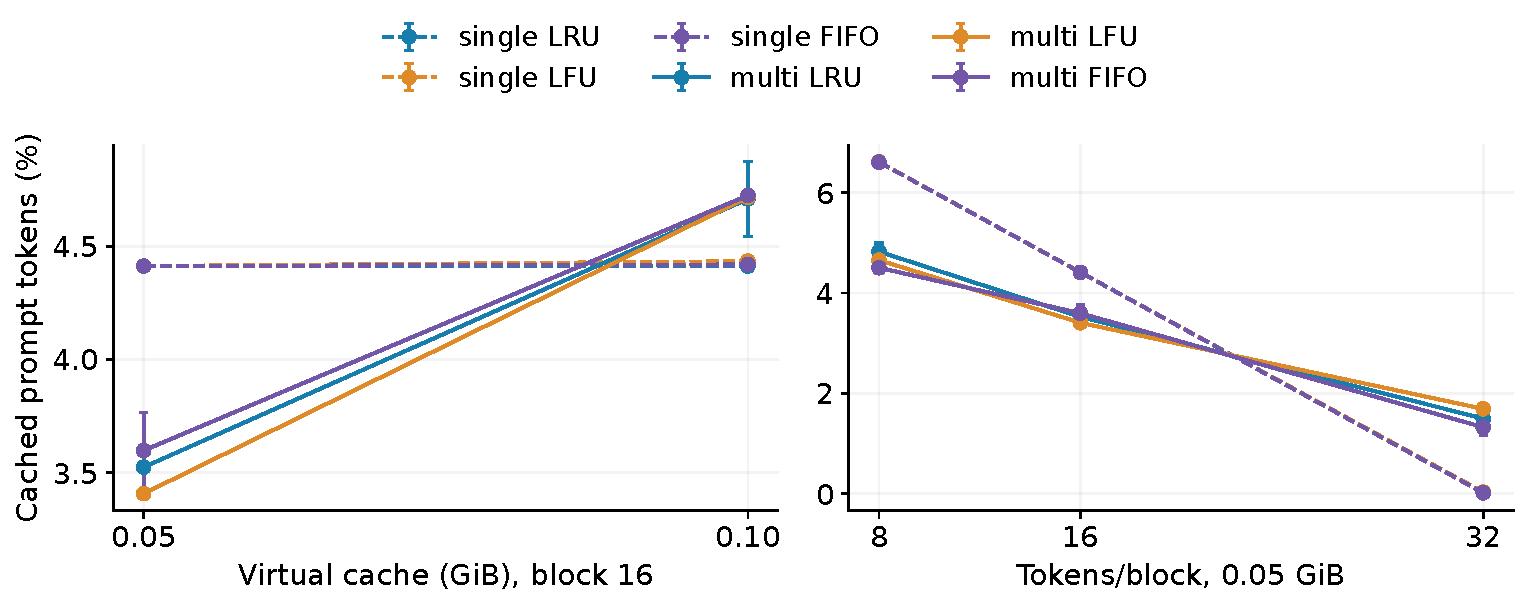
\includegraphics[width=.95\textwidth]{figures/m2_sensitivity.pdf}
\caption{M2 sensitivity under approximately fixed bytes across block sizes. Capacity panel holds block16; granularity panel holds0.05\,GiB. Solid lines: multi; dashed: single. Colors identify policies; points/whiskers are seed means/sample SD. Only two capacities are tested, so a general saturation curve is not established.}
\label{fig:sensitivity}
\end{figure*}

Coarser blocks lose short full-prefix matches and leave longer non-reusable tails. Capacity can preserve more prefixes, but scheduling/preemption may disrupt monotonicity. These proposed mechanisms are not overhead or GPU-efficiency measurements.

\subsection{Separate heterogeneous workloads}
Figure~\ref{fig:task1} uses the validated51-run study (21,834 successful requests, zero failures); the multiprocessing-only transport fix does not alter its direct-mode executor/cache decisions. Coding-agent LRU reaches48.59\% versus35.43\% for LFU and47.35\% for FIFO, approximately13.16pp above LFU. Growing contexts plausibly favor retention of recently added prefixes while frequency can favor older popular blocks; no mechanism ablation proves this explanation.

LFU leads the observed Bailian chat/coder windows (29.52\%/37.28\%) versus LRU28.44\%/35.87\% and FIFO26.75\%/32.88\%. Each has one run, so production-wide superiority is not established. QuALITY FIFO50.35\% exceeds LRU49.25\% and LFU45.54\%, with small repeat counts. AgentBank LRU50.55\% and LFU50.47\% differ by only0.074pp. Mooncake LRU40.27\% and LFU40.25\% nearly tie; FIFO39.72\%. ShareGPT is seed-sensitive; Code Alpaca ties at29.53\% for all policies. Cross-workload capacities/contexts differ, so these establish within-source choices rather than a causal workload ranking.

\begin{figure*}[t]
\centering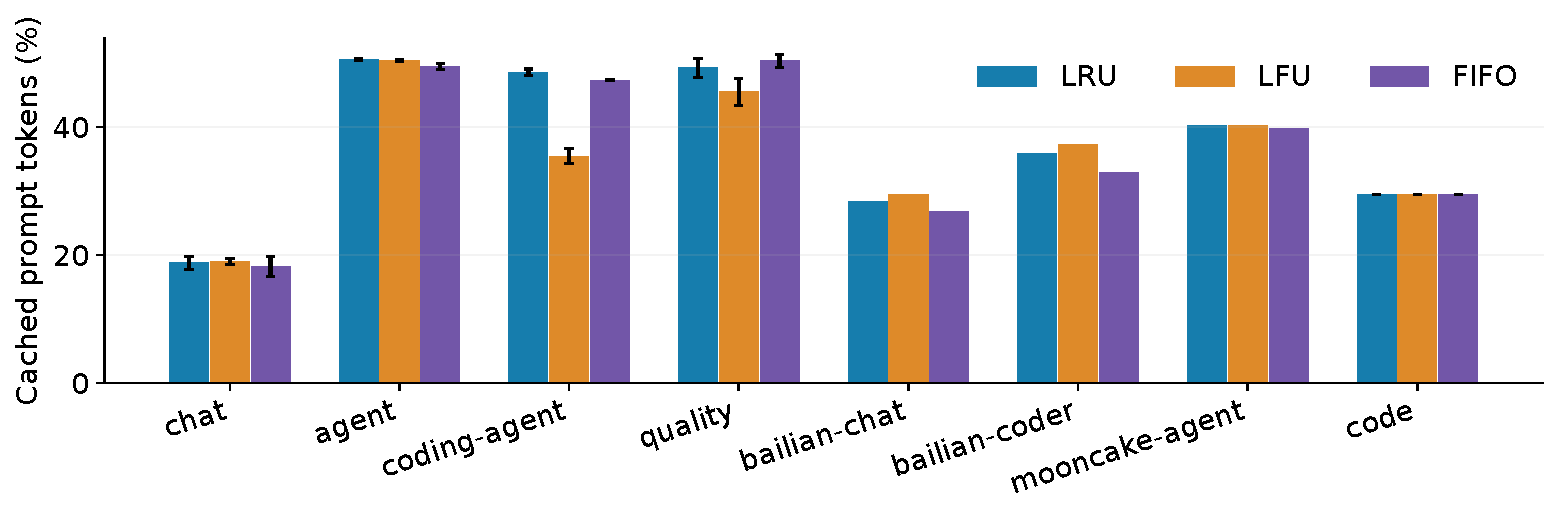
\includegraphics[width=.95\textwidth]{figures/m3_task1.pdf}
\caption{Separate-workload baseline sharing, cache ratio0.25/block16. Whiskers are sample SD for2--3 arrival seeds; production windows have $n=1$ and unknown variability. Highest observed policy and best--second gaps are tabulated in the appendix.}
\label{fig:task1}
\end{figure*}

Representative LRU seed0 CDFs (appendix) show zero-hit blocks ranging from87.23\% in chat to20.37\% in QuALITY. Hit-conditioned wall-clock gaps cannot directly set a universal hold duration.

\begin{figure*}[t]
\centering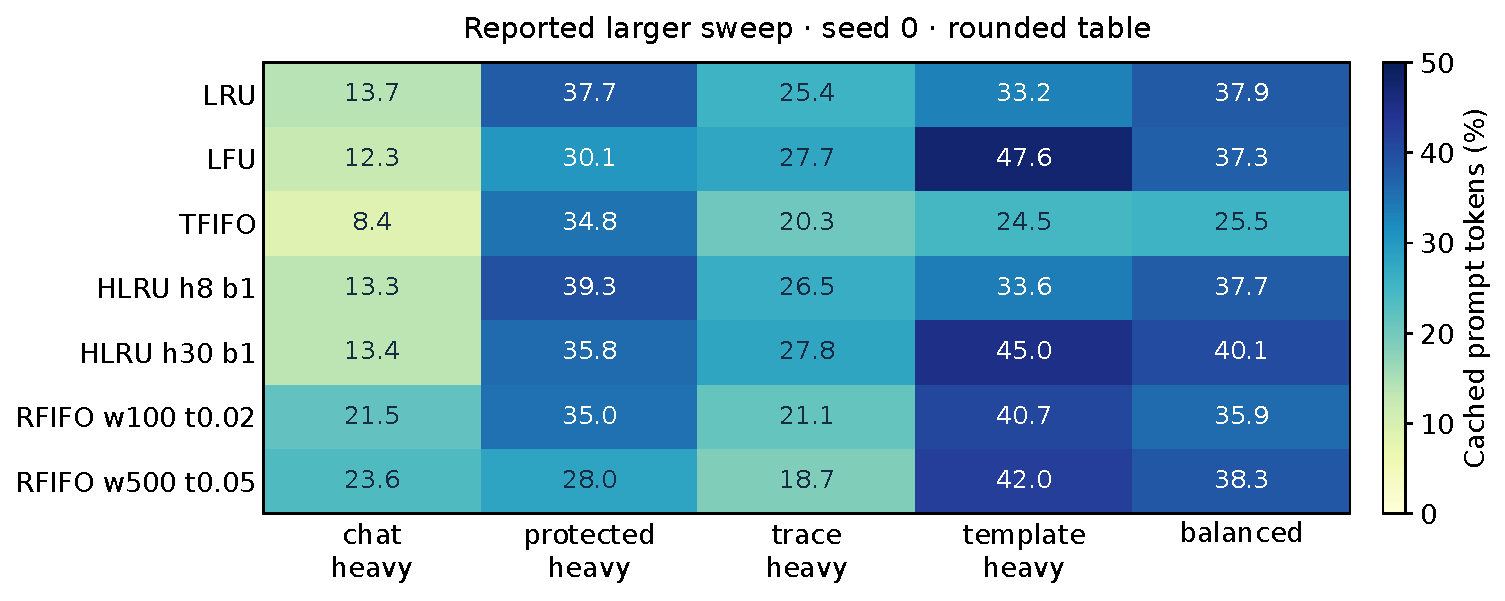
\includegraphics[width=.95\textwidth]{figures/hold_selected.pdf}
\caption{Selected settings from the repository-reported larger sweep. Values are rounded percentages from \texttt{docs/milestone3-task2.md}, not newly executed/raw-validated measurements. Each cell has one seed; close margins lack an uncertainty estimate. Full 25-setting results are in the appendix.}
\label{fig:sweep}
\end{figure*}
\subsection{Mixed-workload policies}
@MIXED_RESULTS@

The aggregate improvements conceal category harm: RFIFO loses14.72\,pp on skewed Bailian-coder and4.83\,pp on equal-token Mooncake versus the strongest respective baseline. These historical runs used the pre-update prepared traces and implementation; they are not reruns of the new commit.

\subsection{Reported hold and admission sensitivity}
Commit \texttt{ad1d826542} reports125 additional cells: five mixtures, 25 settings each, seed0. TLRU/HLRU sweep holds3/8/30\,s and budgets 0.25/1; RFIFO sweeps windows20/100/500 and thresholds2/5/20\%. LRU/LFU/FIFO/TFIFO run once per mix; HFIFO is absent. Capacity is10\% of each distinct working set, block16, concurrency8, think time1\,s. The upstream table reports zero failures and no clamping. Only rounded summaries/plots are available here; raw completion, cohorts and counts are not independently verified or pooled with the175 validated historical runs. Execution order is fixed, not randomized.

@SWEEP_RESULTS@



\section{Discussion and Limitations}
The experiments establish workload/configuration-dependent realized reuse, not one optimal eviction rule. Static labels can preserve useful agent prefixes in one composition while harming a returning conversational category in another; adaptive admission can alter that trade-off without a universal guarantee. Labels are known from data, not predicted. Hold expiration depends on real CPU queuing and HTTP/synthetic delay. Single-seed mixed comparisons, fixed time windows, first-eligible subsets, one cache ratio and absent repeated-seed sensitivity cells limit external validity. Changing mixture also changes selected cohorts and absolute bytes at the fixed ratio, so this is not a composition-only causal ablation. The new sweep explores hold/admission parameters on selected cohorts without held-out evaluation.

The simulator does not model logits, numerical model quality, GPU bandwidth/kernels, real device timing or distributed KV transfer. Reuse scores cannot be converted directly into GPU speedups. CDFs of realized hits exclude missed opportunities; transformed traces omit original agent prompts and shorten production outputs. All trace entries are loaded into memory. The additional sweep has rounded aggregates only; its provenance and lack of raw revalidation are separate from the historical checks. Small margins and selected-parameter means do not establish statistical or out-of-sample superiority.

\section{AI Assistance}
Codex assisted code generation and bug fixes (including multiprocessing labels), tests, experiment scripts, validation, data organization, figures, report and presentation preparation. Automated checks do not establish human review; historical AI use outside this conversation is unconfirmed. Significant user prompts appear in the appendix.

\newpage
\section{Conclusion}
The CPU executor preserves an active online scheduling/cache path while substituting trace tokens for model computation. @CONCLUSION@ The reported sweep further shows parameter-sensitive policy rankings. The findings support conditional policy selection and further controlled validation; they do not establish a GPU performance gain or universally best custom policy.

\clearpage
\bibliographystyle{mlsys2025}
\bibliography{references}
\clearpage
\appendix
\section{Detailed Results and Reproduction}
@APPENDIX_TABLES@

\begin{figure*}[t]\centering
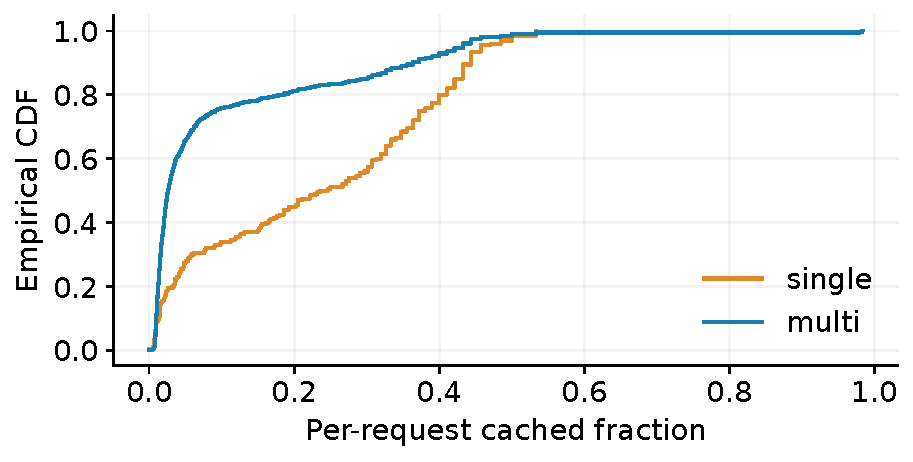
\includegraphics[width=.70\textwidth]{figures/m2_cdf_request.pdf}\hfill
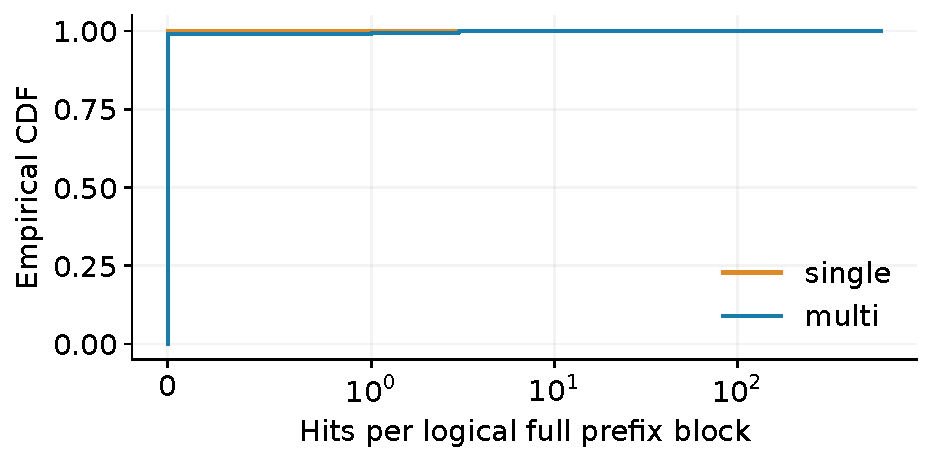
\includegraphics[width=.70\textwidth]{figures/m2_cdf_blocks.pdf}\hfill
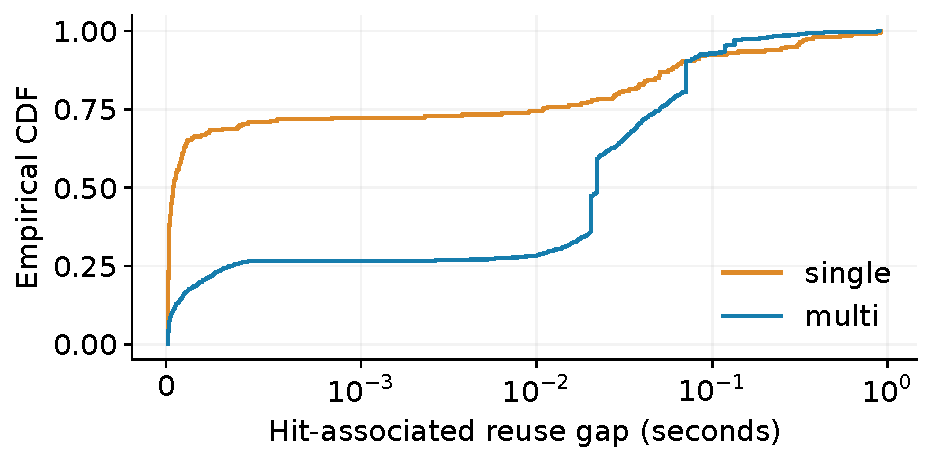
\includegraphics[width=.70\textwidth]{figures/m2_cdf_gaps.pdf}
\caption{M2 descriptive CDFs, LRU/block16/0.05\,GiB/seed0. Request fractions, logical-block hits including zero hits, and successful-hit-associated wall-clock gaps have different populations.}
\end{figure*}
\begin{figure*}[t]\centering
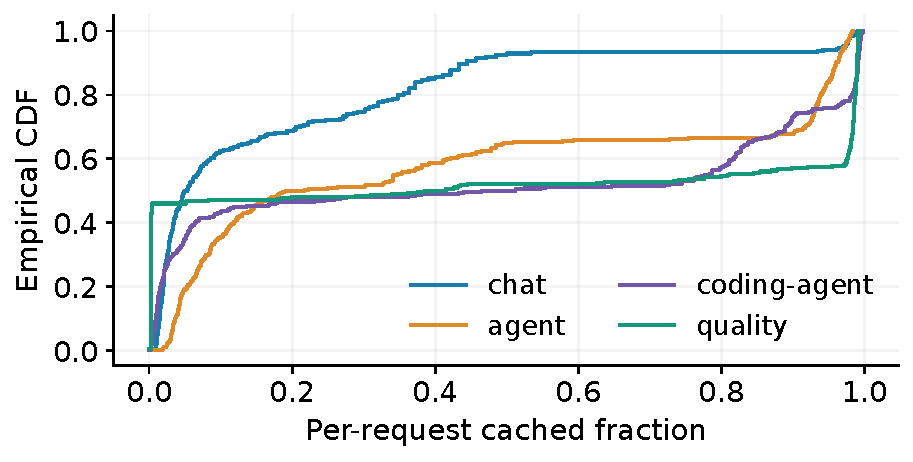
\includegraphics[width=.70\textwidth]{figures/m3_cdf_request.pdf}\hfill
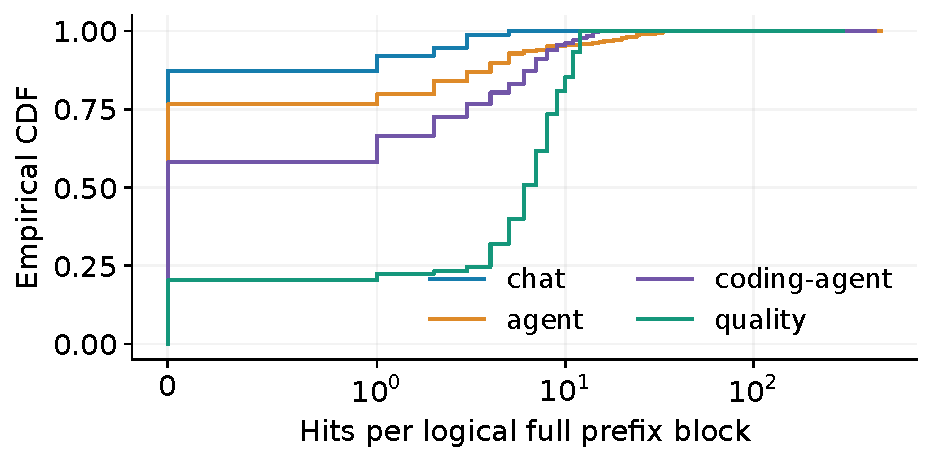
\includegraphics[width=.70\textwidth]{figures/m3_cdf_blocks.pdf}\hfill
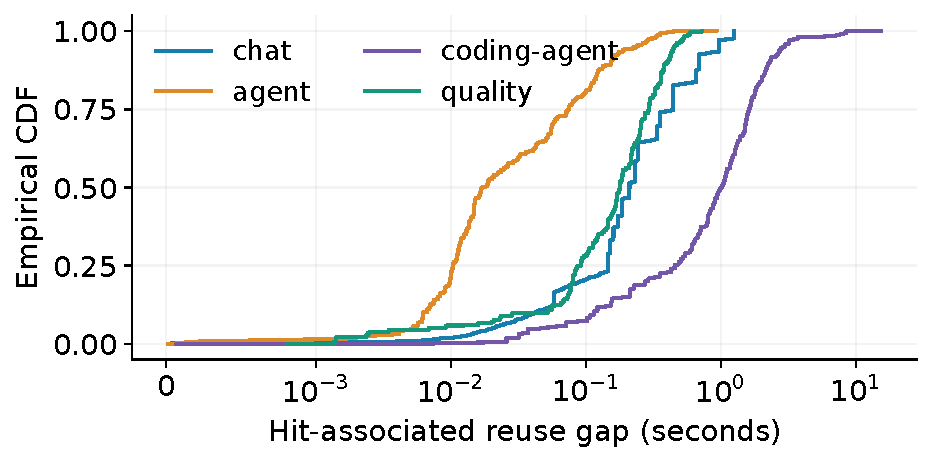
\includegraphics[width=.70\textwidth]{figures/m3_cdf_gaps.pdf}
\caption{Task1 representative LRU seed0 distributions; source-specific contexts/capacities differ. The separate planned-prompt diagnostic uses nominal arrival times and no cache model; it is distinct from these hit-conditioned wall-clock gaps.}
\end{figure*}
\begin{figure*}[t]\centering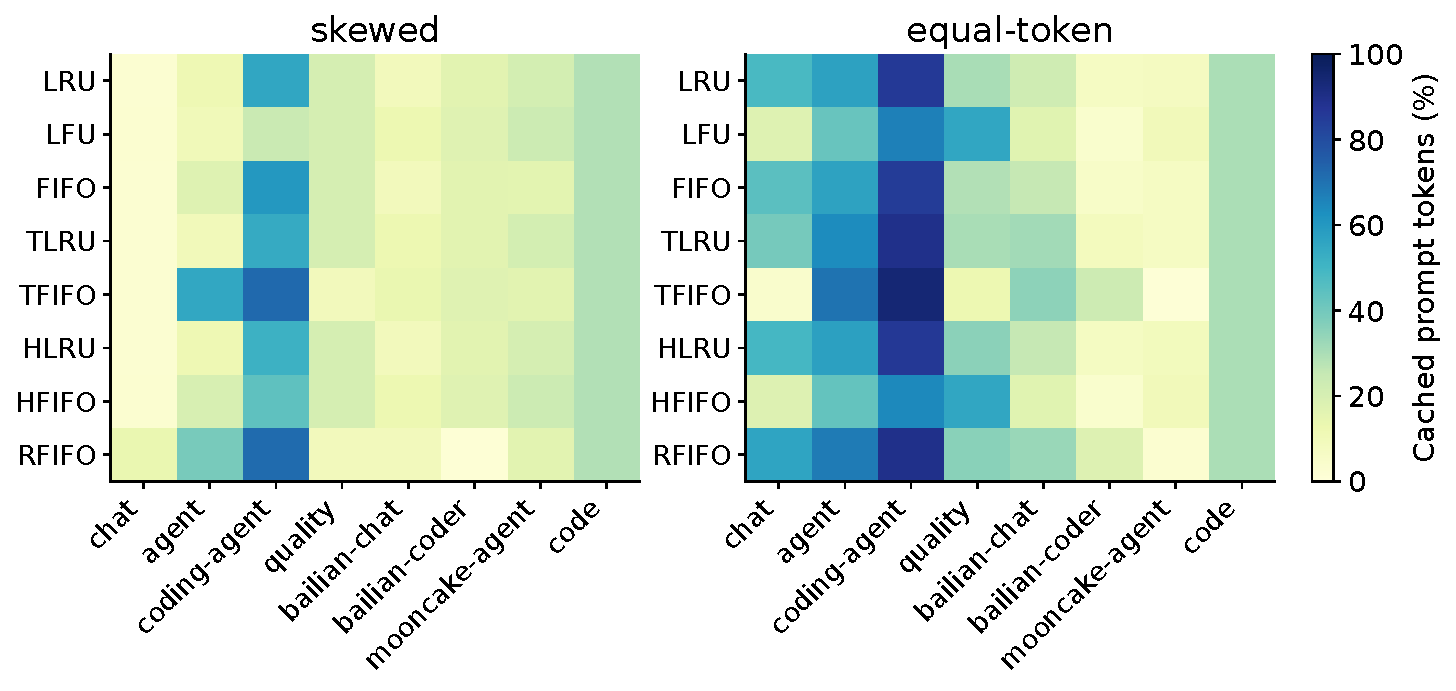
\includegraphics[width=.99\textwidth]{figures/mixed_by_workload.pdf}
\caption{New mixed per-label token-weighted sharing; improvements in an aggregate can conceal harm to individual categories.}
\end{figure*}
\begin{figure*}[t]\centering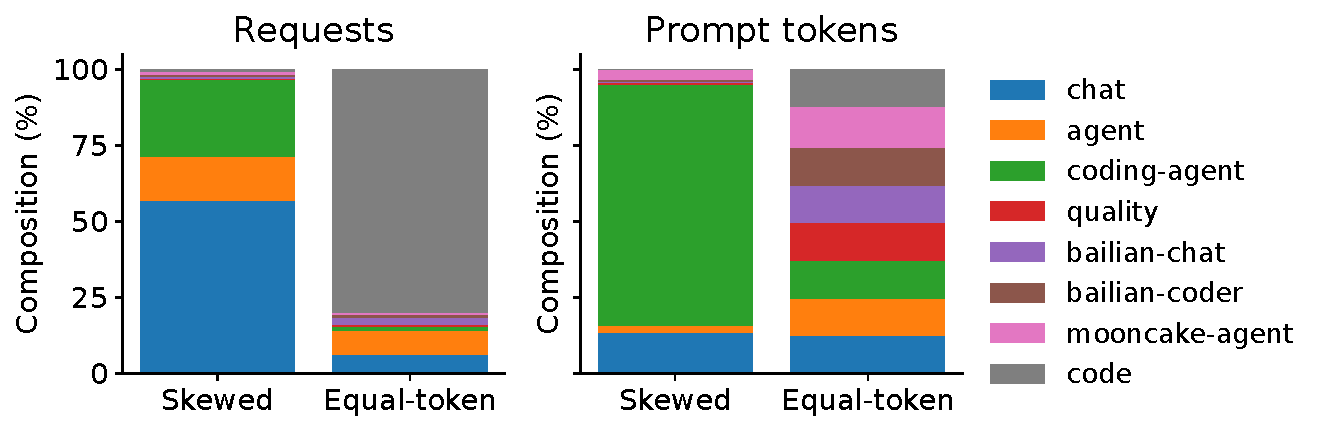
\includegraphics[width=.99\textwidth]{figures/mixed_composition.pdf}
\caption{Request and prompt-token composition are distinct. Equal-token cohorts preserve causal prefixes and overshoot by their last selected turn.}
\end{figure*}

\begin{figure*}[t]\centering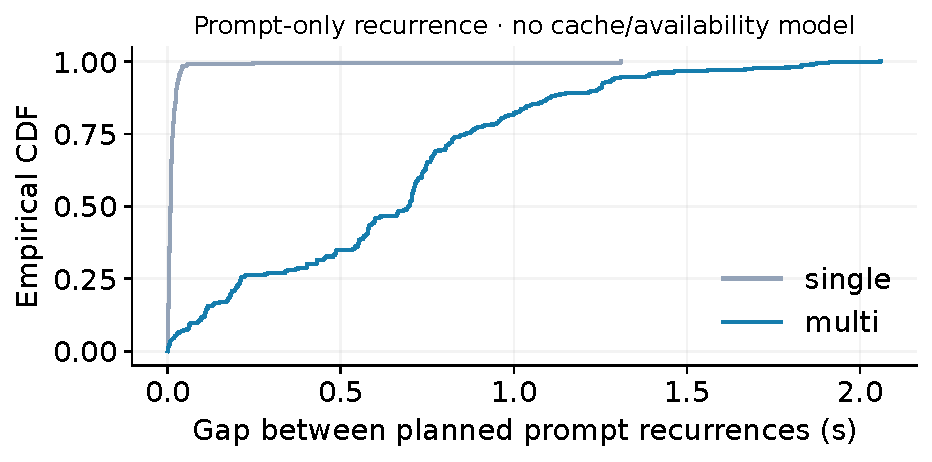
\includegraphics[width=.65\textwidth]{figures/m2_planned_prompt_recurrence.pdf}
\caption{Policy-independent nominal prompt recurrence, M2/block16/seed0. Population: repeated full prompt blocks; no decode-produced blocks, capacity, completion-time availability or actual dispatch model. This is neither a realized-hit CDF nor a full-serving upper bound.}
\end{figure*}
\section{Policy State and Pseudocode}
\begin{table*}[t]\centering\small
\caption{Source-grounded policy comparison. Only unused blocks are candidates; protection is a victim preference, not pinning.}
\begin{tabular}{lp{.34\textwidth}p{.38\textwidth}}\toprule
Policy & Candidate priority / order & State and admission / expiry\\\midrule
LRU & Oldest access; deeper prefix on a tie & Recency metadata\\
LFU & Lowest frequency, then recency/order & Access frequency survives pin/release\\
FIFO & Oldest original insertion serial & Access/pinning does not refresh serial\\
TLRU & Static low, protected, shared tiers; recency & Agent/Bailian labels; shared tier last; hold8\,s and budget1\\
TFIFO & Same static tiers; FIFO & Same labels/shared tier; no hold/budget expiry\\
HLRU & Unhit/expired before fresh reused; recency & First own hit; hold8\,s and budget1\\
HFIFO & Unhit before hit; FIFO & First own hit; no expiry\\
RFIFO & Low before admitted; FIFO & Full100 resolved outcomes/label, $\ge5\%$ hits admit future blocks; no retroactive low-tier promotion\\\bottomrule
\end{tabular}\end{table*}
TLRU: classify each unused cached block as fixed, protected or cross-label shared; demote the oldest protected candidate to fixed competition when expired or above budget; evict the earliest tier's LRU victim. TFIFO: use static label tiers and FIFO serials without time/budget demotion. HFIFO/HLRU: begin unhit; promote on first own reuse; clear hit state on physical reuse; use FIFO or time-limited recency order. RFIFO: resolve a residency once on first hit or unhit eviction; append outcomes to each associated label's last100 entries; admit future blocks when any full label window reaches5\% hits; evict low before admitted tier by insertion order. If no low blocks remain, protected blocks are still evictable. Active pinned blocks are outside the evictor.

Metadata includes label sets, insertion/frequency/hit state, versions and tier heaps; RFIFO additionally uses bounded per-label windows. Typical operations are logarithmic heap operations plus label/window work; lazy stale entries and periodic linear rebuilds mean worst-case latency is not strictly logarithmic. We do not report measured byte/CPU overhead or unavailable promotion counters. Mixed eviction counts come from a successful-allocation wrapper; older runs have no such counter. Full source mapping and limitations are in \texttt{POLICY\_DETAILS.md}.

\section{Team Contributions and Source History}
Author order is Thomas Lin, Yu-Ting Chung, Patrick Chiou and Yu-Xin Lai; all are Rice University affiliates. Complete project history is available and the assigned upstream baseline is an ancestor. Thomas Lin's visible commits cover mixed construction, label transport and custom policies. Yu-Ting Chung's cover original simulator integration/optimization and expanded heterogeneous adapters/traces. Yu-Xin Lai's cover client timing/templates/ID matching, single/multi replay, metrics, FIFO/LFU and M2 sweep automation. Patrick Chiou's cover initial Task1 work and the AI-assisted final report/presentation, testing, bug fix and integration in this session. These are component-level evidence and assigned responsibilities, not effort percentages or presenter assignments. Human review details require confirmation; no corresponding author is designated.

\section{Significant AI Prompts}
The final user instructions asked to complete simulator validation, recover or execute missing M2 and mixed experiments, minimally repair unresolved multiprocessing label transport, preserve original artifacts/history, use the four confirmed authors/emails, produce a six-page MLSys-style main report and update the required15-minute presentation. The presentation supplement specified15 main slides,13min30s timing, approximately1,450--1,600 spoken English words, instructor Q\&A and TA reproduction instructions. Earlier requests asked for initial Task1 code/report, necessary-only Git changes, and a subsequent read-only evidence audit. These are summaries of actual available prompts, not reconstructed historical prompts from other team members. Selected verbatim instructions were: ``Implement the minimal correct fix. Do not simply discard the workload argument or globally disable multiprocessing to hide the problem.'' Another instruction was: ``Do not rerun valid experiments unnecessarily.'' The final request also stated: ``Do not fabricate results, contributions, citations, or validation evidence.'' Complete provided final-task and presentation prompts are archived verbatim in the accompanying \texttt{AI\_PROMPTS.md}; historical prompts from other contributors are not reconstructed.

\begin{figure*}[t]
\centering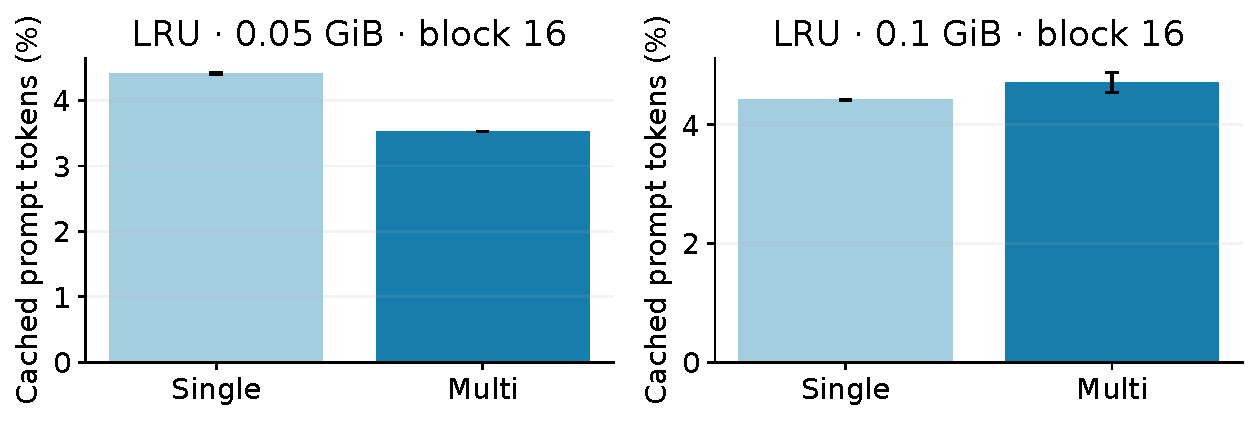
\includegraphics[width=.73\textwidth]{figures/m2_single_multi.pdf}
\caption{Matched single/multi ShareGPT cohorts, LRU/block16. Bars are mean token-weighted sharing and whiskers sample SD over three arrival seeds; capacities are absolute virtual GiB. More conversational history does not imply a larger realized token-weighted fraction under the tested cache and load.}
\label{fig:m2mode}
\end{figure*}
\section{Source Transformations}
Hash traces map to deterministic synthetic token blocks; output filler is capped at32 tokens. Bailian times are scaled by0.25 and Mooncake by0.5; Mooncake has512-token hashes and millisecond timestamps. Agent conversion omits original system/tool schemas; CC conversion excludes thinking/images/sub-agent branches and truncates long contexts. QuALITY interleaves groups of ten articles. These transformations define the studied workload rather than an exact production replica.
\section{New Commit and Reported Sweep Provenance}
The update uses commit \texttt{ad1d826542}, authored by Thomas Lin. It adds configurable RFIFO admission, a five-mixture hold-grid driver, progress/ETA reporting, and filtering of generation-config stop tokens from replies. The sweep test checks grid dimensions, naming/order and progress, not successful completion of125 actual replays. Its resume predicate checks that existing rows are nonempty and successful, without independently checking cohort completeness or source hashes; an interrupted successful prefix could be accepted. The reported zero failures are therefore attributed to the upstream guide, not certified by this update. Existing historical runs remain versioned evidence; changed reply preparation can alter inputs and working sets on a rerun.

The larger sweep has one seed per cell and fixed policy order. Window/threshold choices are selected from the same evaluated mixtures, without a held-out set. Per-mixture cache size and cohort shares differ; the smaller scale is not an independent replication or a composition-only ablation. The guide reports769,775 replayed requests implied by25 times the five cohort sizes, but raw logs and runtime are unavailable here. This count is derived from reported sizes, not added to the independently validated request total.

@SWEEP_TABLES@

\begin{figure*}[t]\centering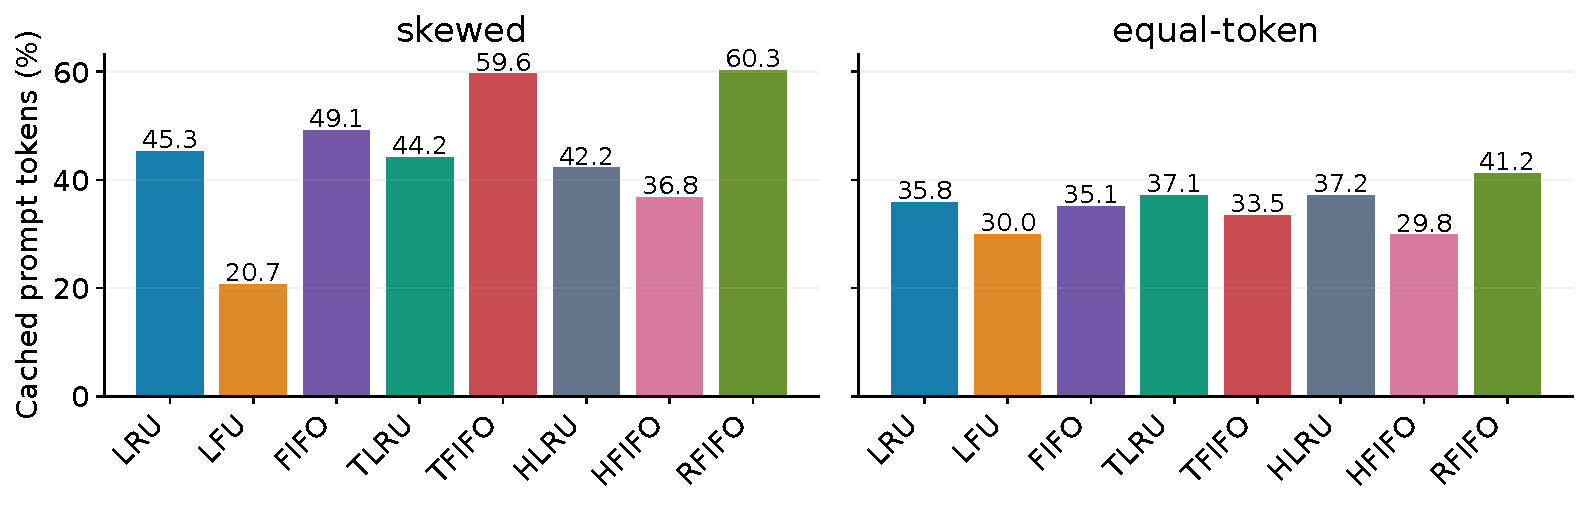
\includegraphics[width=.95\textwidth]{figures/mixed_overall.pdf}
\caption{Historical raw-validated two-mixture comparison, unchanged from the November24 evidence. These runs precede the new reply-preparation changes and are kept separate from the reported sweep.}
\end{figure*}
\begin{figure*}[t]\centering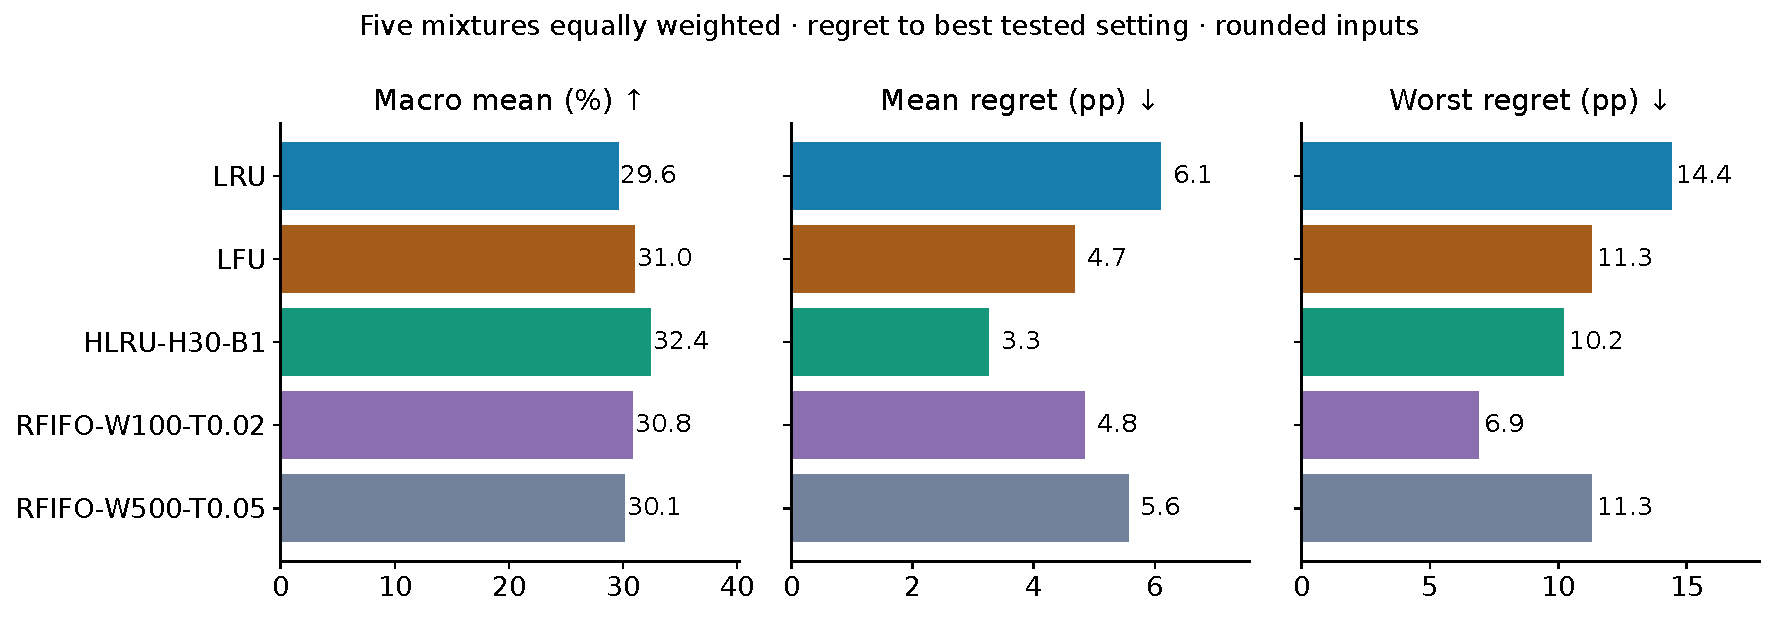
\includegraphics[width=.95\textwidth]{figures/hold_robustness.pdf}
\caption{Derived from the rounded reported table: macro mean weights each of five mixtures equally; regret is the difference from the best tested setting in each mixture. These are descriptive in-sample summaries, not token-pooled scores or uncertainty estimates.}
\end{figure*}

\end{document}
